\documentclass{article}
% translate with >> pdflatex -shell-escape <file>

% This file is used as unit test for pgfplots, copyright by Christian Feuersaenger.
% 
% See
%   http://pgfplots.sourceforge.net/pgfplots.pdf
% for pgfplots.
%
% Any required input files (for <plot table> or <plot file> or the table package) can be downloaded
% at
% http://www.ctan.org/tex-archive/graphics/pgf/contrib/pgfplots/doc/latex/
% and
% http://www.ctan.org/tex-archive/graphics/pgf/contrib/pgfplots/doc/latex/plotdata/

\usepackage{pgfplots}
\pgfplotsset{compat=newest}

\pagestyle{empty}

\usepgfplotslibrary{ternary}

\begin{document}

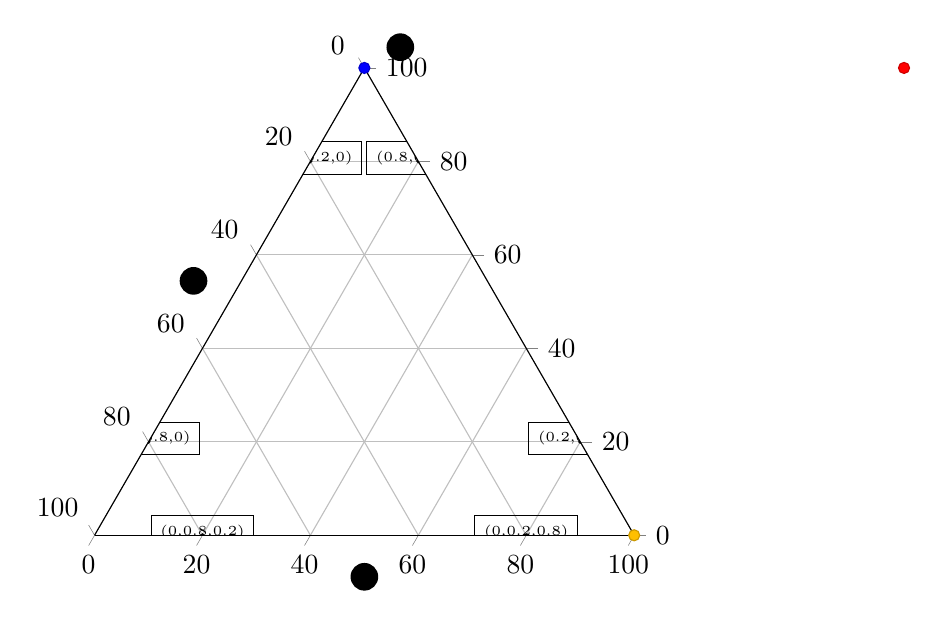
\begin{tikzpicture}
%\tracingmacros=2 \tracingcommands=2
	\begin{ternaryaxis}[
		extra description/.add code={}{%
			\pgfpathcircle
				{\pgfplotsqpointoutsideofaxis{v00}{1}{15pt}}%
				{5pt}%
			\pgfusepath{fill}%
			\pgfpathcircle
				{\pgfplotsqpointoutsideofaxis{0v0}{0.5}{15pt}}%
				{5pt}%
			\pgfusepath{fill}%
			\pgfpathcircle
				{\pgfplotsqpointoutsideofaxis{00v}{0.5}{15pt}}%
				{5pt}%
			\pgfusepath{fill}%
		},
	]

\def\markpoint(#1);{%
	\node[anchor=base,draw=black,font=\tiny] at (axis cs:#1) {(#1)};
	\filldraw (axis cs:#1) circle(0.5pt);
}

	\addplot3[only marks,scatter,point meta=\coordindex] coordinates {
		(1,0,0)
	%	(0,1,0)
		(0,0,1)
		(1,0,1)
	%	(0,0.5,0.5)
	%	(0.5,0.5,0)
	%	(0.5,0,0.5)
	%	(0.33333,0.33333,0.33333)
	};
	%--------------------------------------------------
	% \draw[red] 
	% 	(axis cs:1,0,0) -- 
	% 	(axis cs:0,1,0) --
	% 	(axis cs:0,0,1) -- cycle;
	%-------------------------------------------------- 

		\markpoint(0.8,0,0.2);
		\markpoint(0.8,0.2,0);
		\markpoint(0,0.8,0.2);

		\markpoint(0.2,0,0.8);
		\markpoint(0.2,0.8,0);
		\markpoint(0,0.2,0.8);
	\end{ternaryaxis}
\end{tikzpicture}
\end{document}
